 \documentclass[a4paper,11pt]{article}

\usepackage{amsmath}
\usepackage{amssymb}
\usepackage{amsthm}
\usepackage{graphicx}
\usepackage{caption}
\usepackage{subcaption}

\newtheorem{thm}{Theorem}
\newtheorem{lem}{Lemma}

\newcommand{\beq}{\begin{equation}}
\newcommand{\eeq}{\end{equation}}

\newcommand{\ba}{\begin{array}}
\newcommand{\ea}{\end{array}}

\newcommand{\bea}{\begin{eqnarray}}
\newcommand{\eea}{\end{eqnarray}}

\newcommand{\bc}{\begin{center}}
\newcommand{\ec}{\end{center}}

\newcommand{\ds}{\displaystyle}

\newcommand{\bt}{\begin{tabular}}
\newcommand{\et}{\end{tabular}}

\newcommand{\bi}{\begin{itemize}}
\newcommand{\ei}{\end{itemize}}

\newcommand{\bd}{\begin{description}}
\newcommand{\ed}{\end{description}}

\newcommand{\bp}{\begin{pmatrix}}
\newcommand{\ep}{\end{pmatrix}}

\newcommand{\p}{\partial}
\newcommand{\sech}{\mbox{sech}}

\newcommand{\cf}{{\it cf.}~}

\newcommand{\ltwo}{L_{2}(\mathbb{R}^{2})}
\newcommand{\smooth}{C^{\infty}_{0}(\mathbb{R}^{2})}

\newcommand{\br}{{\bf r}}
\newcommand{\bk}{{\bf k}}
\newcommand{\bv}{{\bf v}}

\setlength{\textheight}{212mm}
\setlength{\textwidth}{165mm}
\topmargin -6mm
\oddsidemargin -6mm


\newcommand{\gnorm}[1]{\left|\left| #1\right|\right|}
\newcommand{\ipro}[2]{\left<#1,#2 \right>}
\title{Elliptical Vortex Patches Under Free Surface Waves}
\date{}
\begin{document}
\maketitle
\begin{abstract}
In this paper, we examine the interactions of freely evolving surfaces in shallow-water scalings with elliptical vortex patches.   The impact of the waves on the stability of the patches is examined, and the manifestation of instabilities in the patches on key surface wave metrics, such as the associated wave spectrum, are studied. 
\end{abstract}
\section*{Model Setup}
In an inviscid, incompressible fluid, we can represent the fluid velocity ${\bf u}(x,z,t)$ generated by a vortex patch characterized by vorticity profile $\omega({\bf x},t)$ over the compact domain $\Omega(t)$ via the integral equation
\[
{\bf u}({\bf x},t) = \int_{\Omega(t)} {\bf K}({\bf x}-\tilde{{\bf x}})\omega(\tilde{{\bf x}},t)d\tilde{x}d\tilde{z} + \nabla \tilde{\phi}, ~ \Delta \tilde{\phi} = 0.
\]
where $\omega$ is the vorticity, and ${\bf K}$ is the standard Biot-Savart law kernel.  The harmonic function $\tilde{\phi}$ is used to address boundary conditions as explained in \cite{saffman}.  An attractive means for discretizing this equation as summarized in \cite{cottet} is to approximate the vorticity $\omega$ by a collection of $N$ point-vortices at positions ${\bf x}_{l}(t)$ via the expansion
\begin{equation}
\omega(\tilde{{\bf x}},t) = \sum_{j=1}^{N} \frac{\Gamma_{j}}{\delta^{2}}\chi\left(\frac{\tilde{{\bf x}}-{\bf x}_{l}(t)}{\delta}\right)
\label{discvort} 
\end{equation}
where $\chi$ is some appropriately chosen mollifier, see \cite{beale}, and $\Gamma_{j}$ is the circulation associated with the point vortex at ${\bf x}_{l}(t)$.  Thus, we can reduce the problem of tracking the evolution of the vortex patch to describing the motion of the point vortices via the system of ODE's
\[
\frac{d{\bf x}_{j}}{dt}  =  \sum_{l\neq j}^{N} \Gamma_{l} {\bf K}_{\delta}\left({\bf x}_{j}-{\bf x}_{l}\right) + \nabla \tilde{\phi}\left({\bf x}_{j},t\right), ~ {\bf K}_{\delta}({\bf x}) = \frac{1}{\delta^{2}}\int_{\mathbb{R}^{2}}{\bf K}({\bf x} - \tilde{\bf x})\chi \left(\frac{\tilde{{\bf x}}}{\delta} \right) d \tilde{{\bf x}}.
\]

\subsection*{Free-Surface Modeling}
However, if the boundary we intend to include is a freely evolving surface, representing waves moving over a vortex patch, this makes the complete description of the fluid difficult.  Thus, in \cite{curtis}, building on the methodology in \cite{afm}, we developed a model which describes the evolution of a free surface $z=H + \eta(x,t)$ and the associated surface velocity $Q(x,t) = \p_{x} \tilde{\phi}(x,\eta(x,t),t)$ moving over a collection of $N$-point vortices.  To do so, we introduce the following non-dimensionalizations
\[
\tilde{x} = \frac{x}{L}, ~\tilde{z} = \frac{z}{H}, ~ \tilde{t} = \frac{\sqrt{gH}}{L} t, ~ \eta = d\tilde{\eta}, ~ \tilde{\phi} = \mu L\sqrt{gH} \tilde{\tilde{\phi}}, ~ \tilde{\Gamma}_{j} = \frac{\Gamma_{j}}{\Gamma},
\]
where we define the non-dimensional parameters
\[
\mu= \frac{d}{H}, ~ \gamma = \frac{H}{L}.  
\]
Note, in this scaling, we see that the vorticity $\omega$ is then scaled as 
\[
\omega = \frac{\mu \sqrt{gH}}{H}\tilde{\omega},
\]
so that by using Stoke's theorem, we see the net circulation $\Gamma$ can be written as 
\[
\Gamma = \mu L \sqrt{gH} \tilde{\Gamma}, ~ \tilde{\Gamma} = \int_{ \tilde{\Omega} } \tilde{\omega} d\tilde{A}.
\]
The rescaled net circulation on the system, $\tilde{\Gamma}$, is a constant of the flow due to Kelvin's theorem.  In these scalings, after dropping tildes, the surface is now at $z = 1 + \mu \eta(x,t)$,  so that by taking $\mu$ and $\gamma$ to be small, we are describing small amplitdue, long-wavelength waves.  If we fix the bottom of our domain at $z=0$ to be a solid boundary, we note that we must modify the Biot-Savart kernel ${\bf K}$ via a method-of-images argument, so that we instead use the kernel $\tilde{{\bf K}}_{\delta}(x,z,\tilde{x},\tilde{z})$ where 
\[
\tilde{{\bf K}}_{\delta}(x,z,\tilde{x},\tilde{z}) = {\bf K}_{\delta}(x-\tilde{x},z-\tilde{z}) - {\bf K}_{\delta}(x-\tilde{x},z+\tilde{z}),
\]
so that by also requiring $\tilde{\phi}_{z}(x,0,t)=0$, we ensure there is zero flow through the solid boundary.  Note, the model equations are somewhat lengthy at this point to write, and they essentially mimic the results in \cite{curtis}, so we omit them for the time being.  Throughout the remainder of this paper, a fourth-order mollifying kernel $\chi$ is used which ensures that over short time scales, the error in the point-vortex method scales like the fourth power of the inter-vortex separation distance if the vortices are affixed to a regular mesh.  

With this idea of placing vortices on a uniform mesh in mind, the error in this approximation can be understood as a balance between the spacing of the point-vortices and the choice of mollifier, see the proofs in \cite{cottet}.  There, a vague notion of a ``particle overlap" critierion is introduced, which while somewhat conceptually pleasing, is difficult to apply in practice.  A more straightforward understanding of error for this method is by way of interpolation.  To wit, if we start with a regularly spaced array of points ${\bf x}_{l}(0)$ then as the flow evolves in time, shearing will distort this grid, clustering points in some regions and making them relatively sparse in others.  

Thus, the error associated with using said points in an interpolatory scheme can become highly irregular, representing the overall error in the method.  We therefore employ the regridding scheme detailed in \cite{cottet}, whereby the distorted points are interpolated back to a uniform mesh at a fixed number of time steps in the numerical scheme.  This does increase the total number of vortices in the simulation over time, necessitating the use of Fast-Multipole Methods (FMMs) to maintain the overall speed of the simulation.  With these methods in place though, we can ensure the accuracy of the complicated and thin filament formation seen in the following simulations.      

\section*{Validation}
We use the circularly symmetric, compactly supported vorticity profile
\[
\omega(r) = \omega_{0}\left\{  \ba{rl} \left(1-\frac{r^{2}}{R_{v}^{2}}\right)^{3} & r\leq R_{v} \\ 0 & r>R_{v} \ea\right.
\] 
for the purposes of validation.  In the absence of any boundaries or free-surfaces, this profile should effectively remain constant in time, thereby allowing us to determine the accuracy of our point-vortex with regridding method.  {\bf I'll put the obligatory figures here later, but it all works.}
\section*{Numerical Experiments}
We now turn to the study of the Kirchoff elliptical vortices \cite{mitchell,crosby} and how their dynamics is influenced by the impact of free surface waves.  In the shallow water scalings used above, a Kirchoff elliptical vortex is a vortex patch with constant vorticity $\omega$ and support within the elliptical disc
\[
\left(\frac{x}{a}\right)^{2} + \gamma^{2}\left(\frac{z-z_{c}}{b} \right)^{2} \leq 1.
\]
It is a now classical result, see \cite{mitchell} for details, that in the absence of outside influences, the patch simply rotates with $\dot{a}=\dot{b}=0$ and the angle describing the rotation being given in these coordinates by 
\[
\dot{\theta} = \frac{\mu}{\gamma} \frac{\omega ab}{(a+b)^{2}}.
\]
This is an idealized result however since if the ratio of major to minor axes is greater than three, the patch becomes unstable.  This instability manifests as the production of tendrils growing from the patch which, in a certain limit, provides an approximation to eventual vortex shedding.  

To generate numerical simulations then, we first note that the discontinuity in the vorticity makes point-wise interpolation impractical.  Therefore, we model the vorticity as 
\[
\omega(x,z) = \omega_{0}\mbox{exp}\left(\log(\mbox{eps}) \left(\left(\frac{x}{a}\right)^{2} + \gamma^{2}\left(\frac{z-z_{c}}{b} \right)^{2}\right)^{10}\right)
\]
where $\mbox{eps}$ denotes machine precision, which is approximately $2\times 10^{-16}$ on most 64-bit computers.  Note, this vorticity profile only has support on the original elliptical disc, has essentially constant vorticty $\omega_{0}$ throughout the elliptical disc, but smoothly vanishes at the boundary.  

The vorticity function is sampled over a uniform mesh of step size $dx = dz = 2.5 \times 10^{-3}$, and the initial circulations $\Gamma_{j}$ are found by solving the linear system in Equation \eqref{discvort}.  We use a fourth order Runga-Kutta scheme with a time step of $dt = 10^{-1}$ and an integrating factor to address the dispersion introduced by the free-surface.  The regridding is done every five time steps to address the shear-induced distortion of the relative separation of the point-vortices.  To cope with the increasing number of vortices this introduces, we use a FMM to make the evaluation of the velocities induced by the vortices scale like $\mathcal{O}(N\log(N))$.  We note that in order to improve performance, we remove the mollification over the well-separated vortices in the FMM scheme, saving mollification only between nearest-neighbors in the FMM scheme.  The impact of this choice on the physics is negligible.  Lastly, a pseudo-spectral in space scheme is used with $K_{T}=256$ modes over a domain size of $L=2$, so that the free surface is sampled at every $1/128$ steps.   

We now present results for which $a=2$, $b=1$, $z_{c}=.35$, $\omega_{0}=5$.  This puts us well within the stability regime for a patch, which is well-reflected in the patch dynamics seen in Figure \ref{fig:vortprofilesstab}.  Note, if Figures \ref{fig:vortprofilesstab} (c) and (d), while the free surface is removed, the solid boundary along $z=0$ is still present, thereby allowing for a relatively direct examination of the impact of the free surface on the patch.  We see that the surface induces relatively significant deformations of the patch, though it does not seem to induce strong enough variations to manifest instabilities.  
\begin{figure}[!h]
\begin{tabular}{cc}
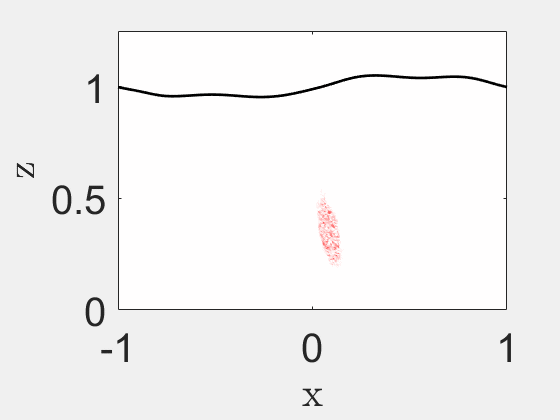
\includegraphics[width=.5\textwidth]{rows_200_cols_400_K_128_mu_pt01_gam_pt031623_F_015895_tf_5_elp_2.png}	& 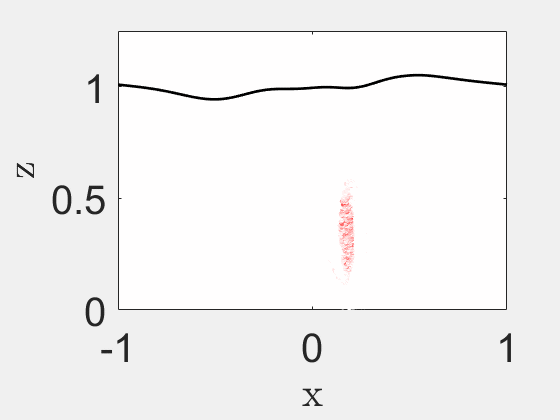
\includegraphics[width=.5\textwidth]{rows_200_cols_400_K_128_mu_pt01_gam_pt031623_F_015895_tf_10_elp_2.png}\\
(a) $t_{f}=5$ & (b) $t_{f}=10$\\
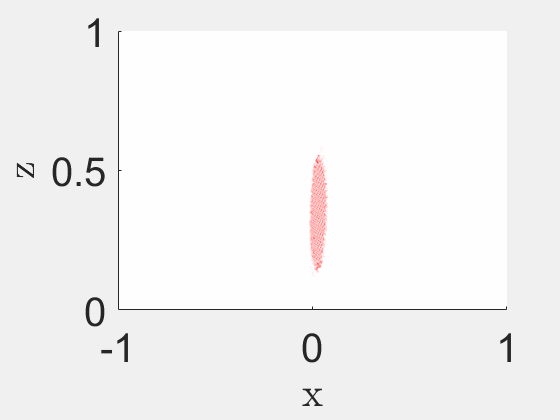
\includegraphics[width=.5\textwidth]{rows_200_cols_400_mu_pt01_gam_pt031623_F_015895_tf_5_elp2.png}	& 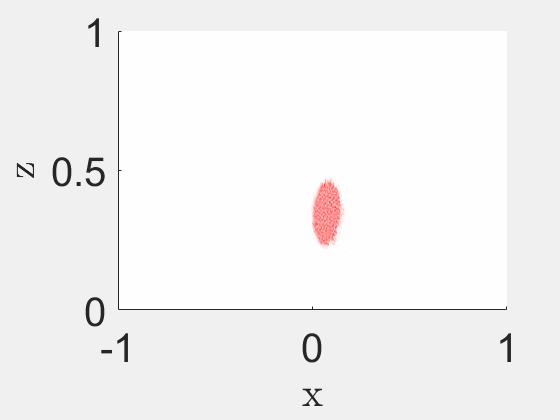
\includegraphics[width=.5\textwidth]{rows_200_cols_400_mu_pt01_gam_pt031623_F_015895_tf_10_elp2.png}\\
(c) $t_{f}=5$& (d) $t_{f}=10$
\end{tabular}	
\caption{Plots of an elliptical vortex patch with $a=2$, $b=1$, $\omega_{0}=5$ with a free-surface present ((a) and (b)) and without one present ((c) and (d)).  }
\label{fig:vortprofilesstab}
\end{figure}  

In contrast to the stable case above, we now let $a=3$, $b=1$, $z_{c}=.35$, $\omega_{0}=5$, which puts us on the cusp of  instability for a patch.  As we see in Figure \ref{fig:vortprofilesinstab}, this instability does not appear unless the free-surface is there to act as a pressure perturbation (compare Figures \ref{fig:vortprofilesinstab} (a) and (b) to Figures \ref{fig:vortprofilesinstab} (c) and (d)).  As can be seen, the impact of the free-surface is more significant than in the stable case seen above.  In particular, we see that filaments of vorticity are produced by the pressure fluctuations corresponding to the oscillations of the surface.  
\begin{figure}[!h]
\begin{tabular}{cc}
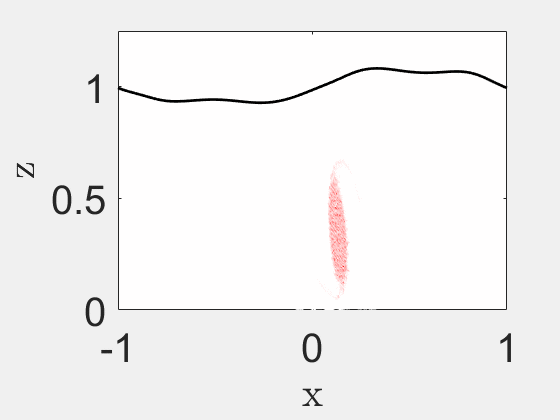
\includegraphics[width=.5\textwidth]{rows_200_cols_400_K_128_mu_pt01_gam_pt031623_F_023843_tf_5.png}	& 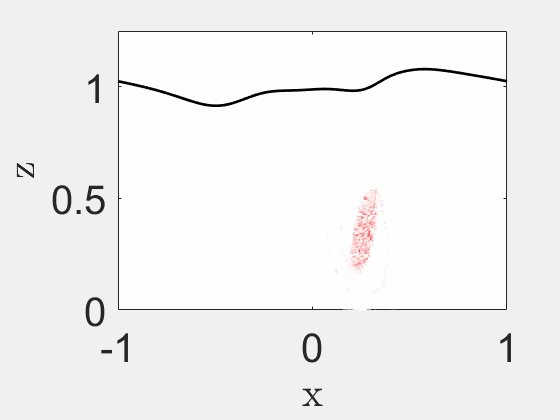
\includegraphics[width=.5\textwidth]{rows_200_cols_400_K_128_mu_pt01_gam_pt031623_F_023843_tf_10.png}\\
(a) $t_{f}=5$ & (b) $t_{f}=10$\\
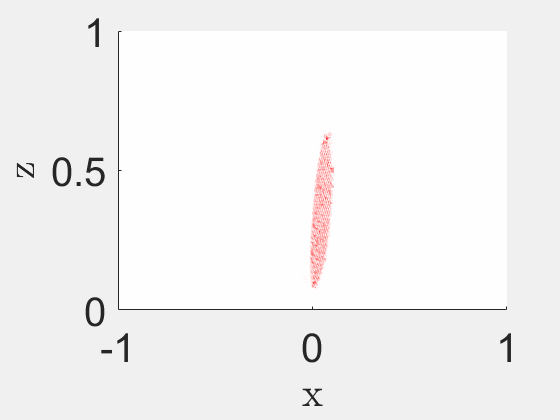
\includegraphics[width=.5\textwidth]{rows_200_cols_400_mu_pt01_gam_pt031623_F_023843_tf_5.png}	& 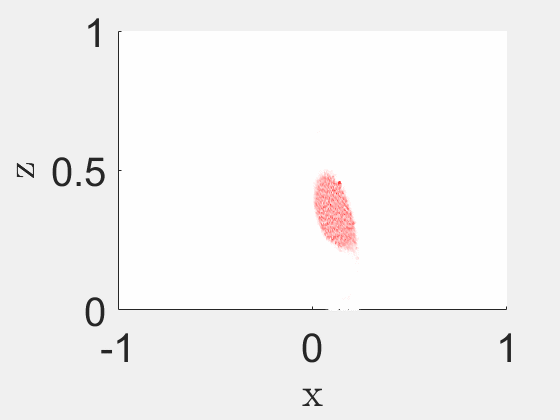
\includegraphics[width=.5\textwidth]{rows_200_cols_400_mu_pt01_gam_pt031623_F_023843_tf_10.png}\\
(c) $t_{f}=5$& (d) $t_{f}=10$
\end{tabular}	
\caption{Plots of an elliptical vortex patch with $a=3$, $b=1$, $\omega_{0}=5$ with a free-surface present ((a) and (b)) and without one present ((c) and (d)).  }
\label{fig:vortprofilesinstab}
\end{figure}  
\bibliography{waves_over_vortices}
\bibliographystyle{unsrt}
\end{document}